\chapter{Evaluation}\label{ch:evaluation}
%klare begründung => Anforderung erfüllt ja oder nein


\section{RANSAC Algorithm}

\subsection{Tests on singular synthetic cube}

A unit cube will be used as a test object to evaluate the RANSAC algorithm.
The cube has been generated with a side length of 1 and a sampling rate of 0.01.
This would equate to a cube with a side length of 1m and a distance of 1cm between points in the real world,
which is comparable to what is provided by the Raw Depth API\@.

\subsubsection{Resilience to Noise}
In figure~\ref{fig:test-noise}, the unit cube is shown with varying noise levels using gaussian noise.
The noise level is defined as the standard deviation of the noise added to the points.

With a noise level of 0.01, the cube is perfectly reconstructed.
Increasing the noise level to 0.02, the cube is still recognized mostly correctly.
Starting from noise level to 0.03, the default parameters do not yield correct results.
To achieve correct results, the epsilon parameter of the RANSAC algorithm has to be increased to 0.2.
This leads to 6 faces being recognized correctly, but some points not being assigned to the correct faces,
as the with each primitive extraction pass, points are extracted that lie within 0.2 of the recognized plane.


\begin{figure}[p]
    \centering
    % First row
    \begin{subfigure}[b]{0.25\textwidth}
        \centering
        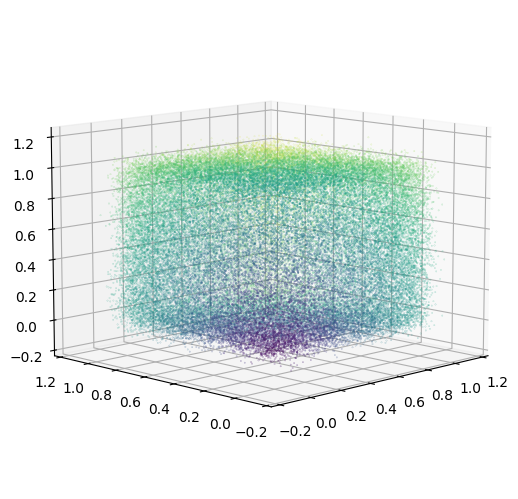
\includegraphics[width=0.9\linewidth]{python/plots/cube_points/data/cube_points}
    \end{subfigure}%
    \begin{subfigure}[b]{0.25\textwidth}
        \centering
        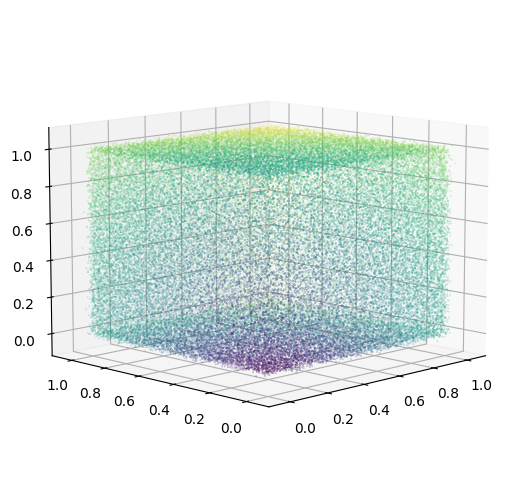
\includegraphics[width=0.9\linewidth]{python/plots/cube_points/data/noise/cube_points_noise_01}
    \end{subfigure}%
    \begin{subfigure}[b]{0.25\textwidth}
        \centering
        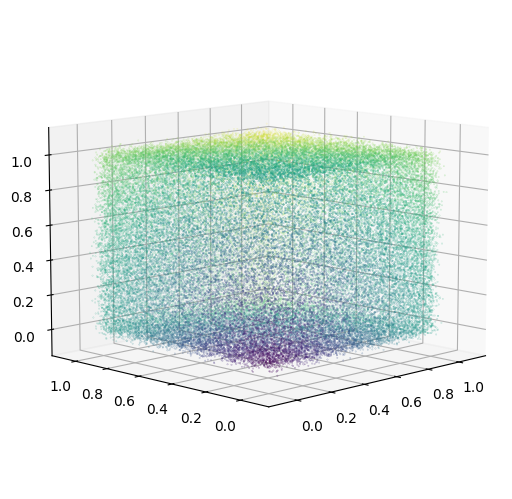
\includegraphics[width=0.9\linewidth]{python/plots/cube_points/data/noise/cube_points_noise_02}
    \end{subfigure}%
    \begin{subfigure}[b]{0.25\textwidth}
        \centering
        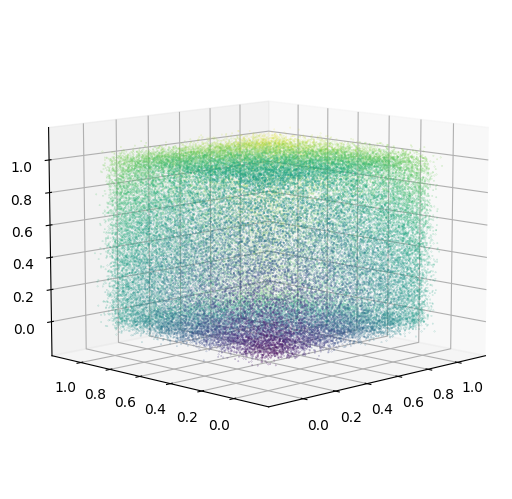
\includegraphics[width=0.9\linewidth]{python/plots/cube_points/data/noise/cube_points_noise_03}
    \end{subfigure}%

%    \vspace{0.5em}

    \begin{subfigure}[b]{0.25\textwidth}
        \centering
        
\includegraphics[width=0.9\linewidth]{python/plots/cube_points/data/cube_points_primitives}
        \caption{Noise level 0.00}
    \end{subfigure}%
    \begin{subfigure}[b]{0.25\textwidth}
        \centering
        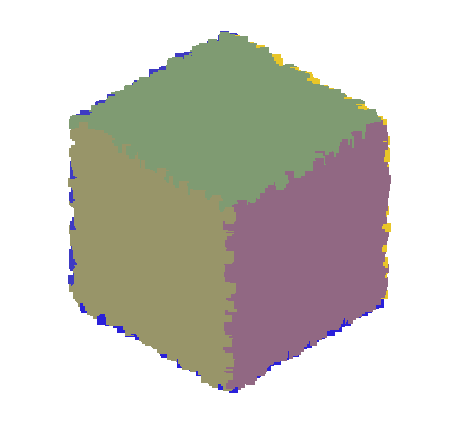
\includegraphics[width=0.9\linewidth]{python/plots/cube_points/data/noise/cube_points_noise_01_primitives}
        \caption{Noise level 0.01}
    \end{subfigure}%
    \begin{subfigure}[b]{0.25\textwidth}
        \centering
        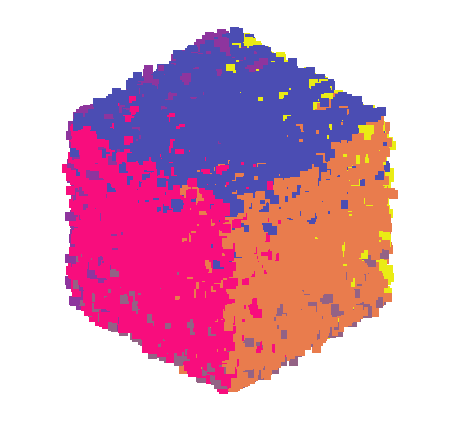
\includegraphics[width=0.9\linewidth]{python/plots/cube_points/data/noise/cube_points_noise_02_primitives}
        \caption{Noise level 0.02}
    \end{subfigure}%
    \begin{subfigure}[b]{0.25\textwidth}
        \centering
        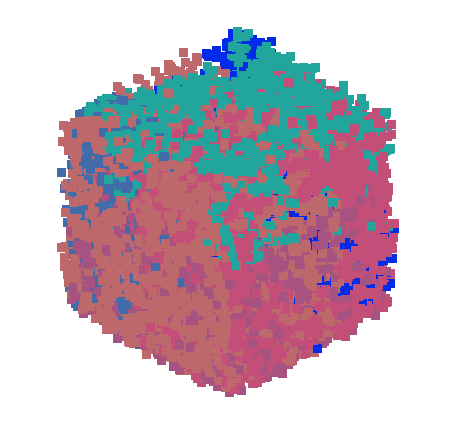
\includegraphics[width=0.9\linewidth]{python/plots/cube_points/data/noise/cube_points_noise_03_primitives}
        \caption{Noise level 0.03}
    \end{subfigure}%

    \caption{Unit cube with varying noise level}
    \label{fig:test-noise}
\end{figure}

\subsubsection{Resilience to Missing Data}

As a big problem of depth from motion techniques is the lack of depth information in areas with minimal texture,
the resilience to missing data is crucial.
In figure~\ref{fig:test-missing}, points towards the center of the cubes surfaces have been removed.
This mimics the structure of real world data from the Depth API,
as edges are often detected more accurately than surfaces.
%TODO: citation needed
To achieve this, points have been removed with an increasing probability based on the
quadratic distance to the center of the face the points belongs to.

The algorithm is able to correctly recognize the faces of the cube with a missing level up to 24.
With a missing level of 48, the algorithm still detects the planes, but doesn't assign all points to the faces.
With increasing missing level, the n parameter, which defines the minimum number of points required to fit a primitive,
is also required to be lowered.
In real world applications this would lead to more false detections, primitives being detected where there are none.

%Given a point $x$ with coordinates $(x_1, x_2, x_3)$, edge length $l$, and missing data rate $r$,
%the distance to the closest edge can be calculated as |
%
%As the cube is centered at the origin and aligned with the axis, the absolute of one coordinate will always equal $l/2$.
%By filtering out this coordinate, the point $x$ can be projected onto the plane of the cube,
%resulting in point $x'$ with coordinates $(x'_1, x'_2)$.
%
%The probability $p$ of a point being removed can then be calculated as

%\begin{equation}
%    p = \left(\frac{\sqrt{(l/2 - |x'_1|) \cdot (l/2 - |x'_2|)}}{l / 2}\right)^2 \cdot r
%\end{equation}

\subsubsection{Resilience to Noise and Missing Data}

When combining both noise and missing data, the quality of the detection is much worse.
In figure~\ref{fig:test-both}, the cube is shown with a noise level of 0.01 and varying missing levels.
With noise level 0.01 and missing level 6, the cube is still recognized correctly.
With missing level 12, more than 6 faces are being recognized, but all the points are still assigned to primitives.
This is explained by the fact that the parameterization of the planes is not accurate enough to fit all the points of the planes.
Thus, the algorithm only fits a subset of the points to the primitive and will create a new parameterization
for the remaining points.
To achieve results with these conditions, the epsilon parameter had to be increased to 0.015 to achieve any results at all.
Using a noise level of 0.02 with missing data yields no satisfactory results, even with tweaking the parameters.

\begin{figure}[p]
    \centering
    % First row
    \begin{subfigure}[b]{0.25\textwidth}
        \centering
        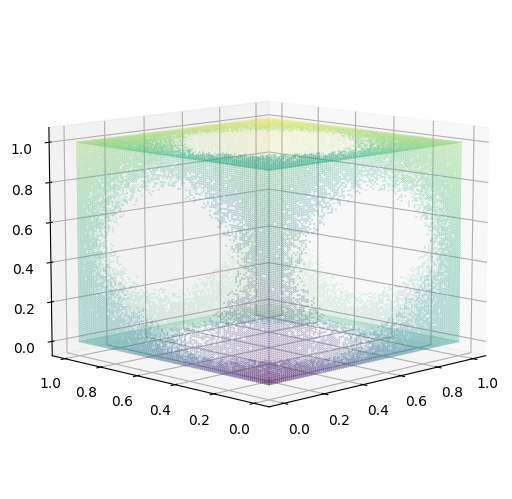
\includegraphics[width=0.9\linewidth]{python/plots/cube_points/data/missing/cube_points_missing_6_0}
    \end{subfigure}%
    \begin{subfigure}[b]{0.25\textwidth}
        \centering
        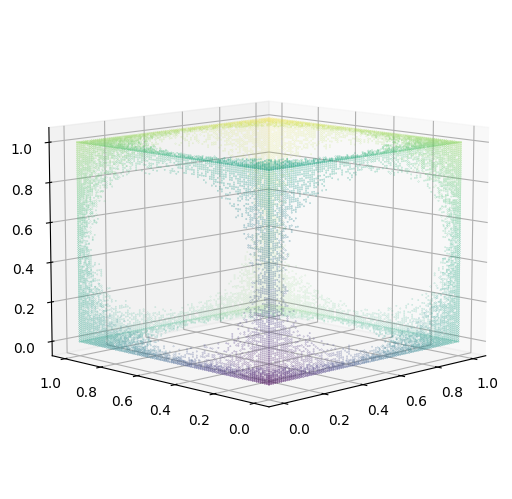
\includegraphics[width=0.9\linewidth]{python/plots/cube_points/data/missing/cube_points_missing_12}
    \end{subfigure}%
    \begin{subfigure}[b]{0.25\textwidth}
        \centering
        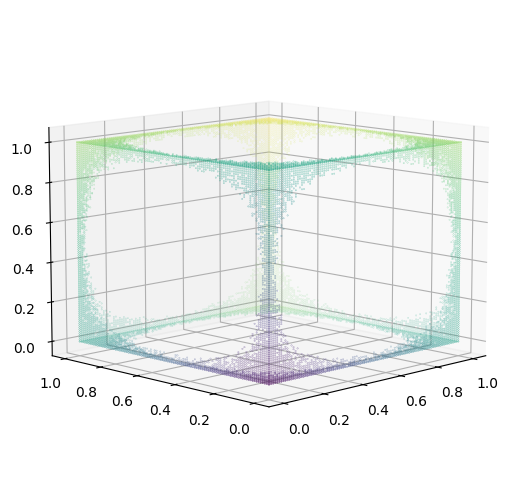
\includegraphics[width=0.9\linewidth]{python/plots/cube_points/data/missing/cube_points_missing_24}
    \end{subfigure}%
    \begin{subfigure}[b]{0.25\textwidth}
        \centering
        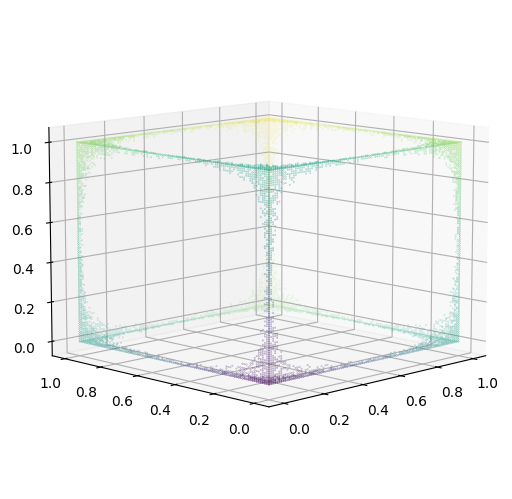
\includegraphics[width=0.9\linewidth]{python/plots/cube_points/data/missing/cube_points_missing_48}
    \end{subfigure}%

%    \vspace{0.5em}

    \begin{subfigure}[b]{0.25\textwidth}
        \centering
        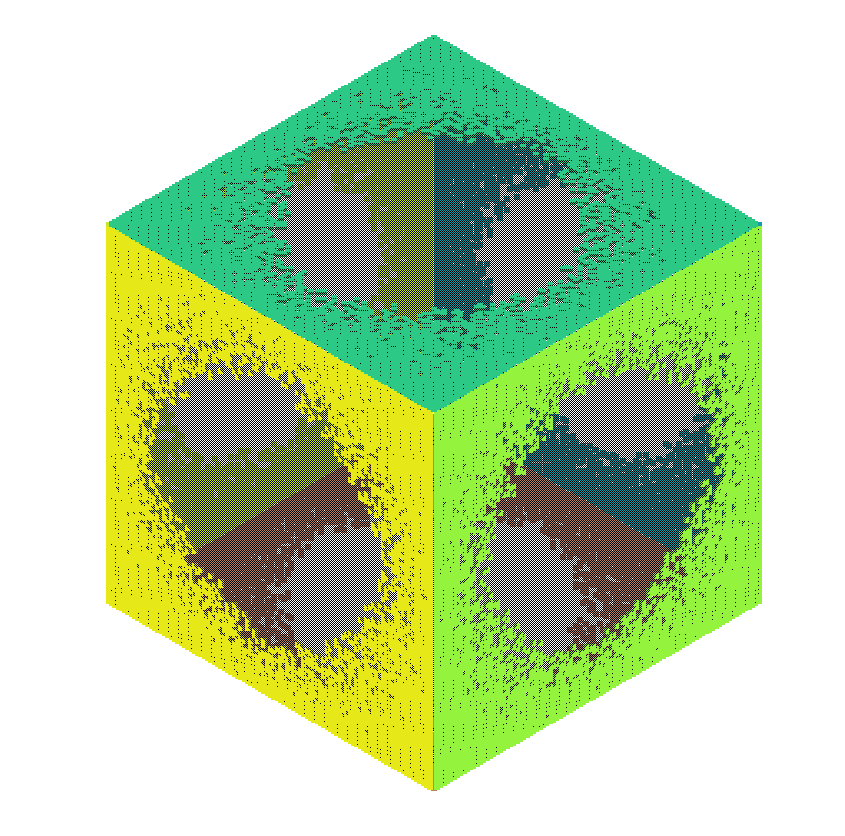
\includegraphics[width=0.9\linewidth]{python/plots/cube_points/data/missing/cube_points_missing_6_primitives}
        \caption{Missing level 6}
    \end{subfigure}%
    \begin{subfigure}[b]{0.25\textwidth}
        \centering
        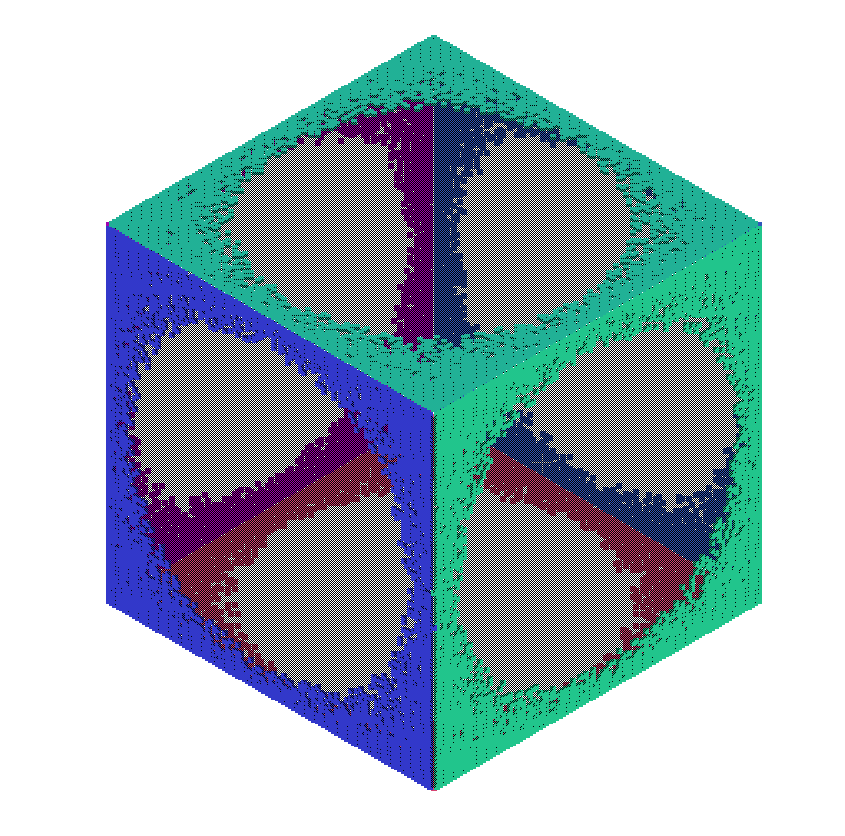
\includegraphics[width=0.9\linewidth]{python/plots/cube_points/data/missing/cube_points_missing_12_primitives}
        \caption{Missing level 12}
    \end{subfigure}%
    \begin{subfigure}[b]{0.25\textwidth}
        \centering
        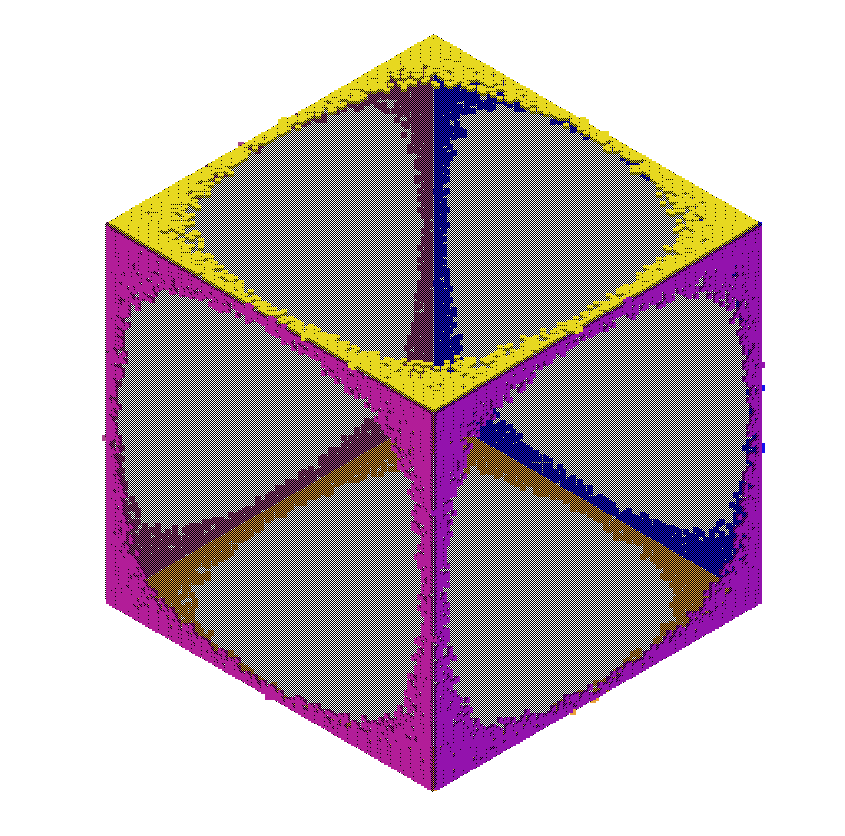
\includegraphics[width=0.9\linewidth]{python/plots/cube_points/data/missing/cube_points_missing_24_primitives}
        \caption{Missing level 24}
    \end{subfigure}%
    \begin{subfigure}[b]{0.25\textwidth}
        \centering
        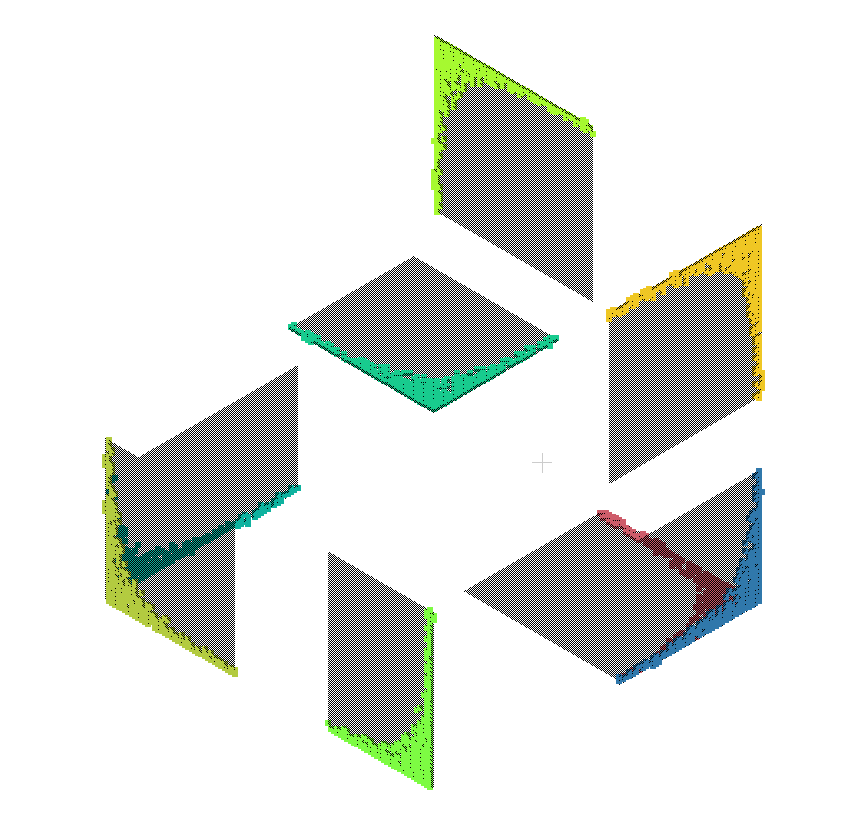
\includegraphics[width=0.9\linewidth]{python/plots/cube_points/data/missing/cube_points_missing_48_primitives}
        \caption{Missing level 48}
    \end{subfigure}%

    \caption{Unit cube with varying missing level}
    \label{fig:test-missing}
\end{figure}

\begin{figure}[ht!]

    \centering
    % First row
    \begin{subfigure}[b]{0.25\textwidth}
        \centering
        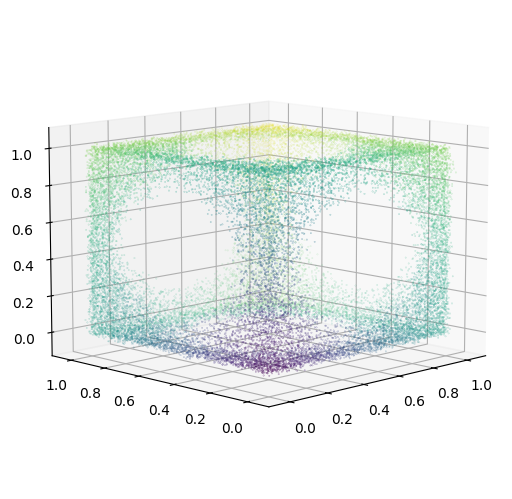
\includegraphics[width=0.9\linewidth]{python/plots/cube_points/data/matrix/cube_points_m6_n01}
    \end{subfigure}%
    \begin{subfigure}[b]{0.25\textwidth}
        \centering
        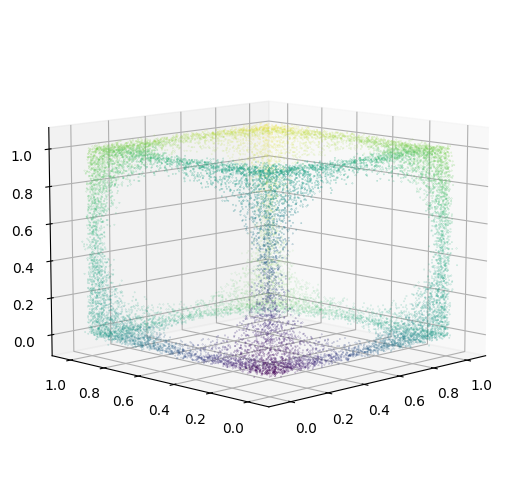
\includegraphics[width=0.9\linewidth]{python/plots/cube_points/data/matrix/cube_points_m12_n01}
    \end{subfigure}%
    \begin{subfigure}[b]{0.25\textwidth}
        \centering
        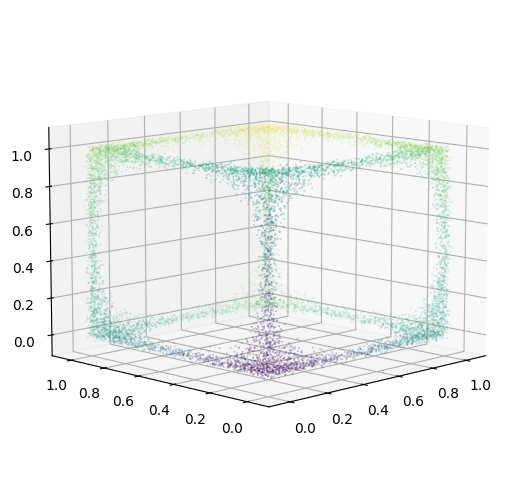
\includegraphics[width=0.9\linewidth]{python/plots/cube_points/data/matrix/cube_points_m24_n01}
    \end{subfigure}%

%    \vspace{0.5em}

    \begin{subfigure}[b]{0.25\textwidth}
        \centering
        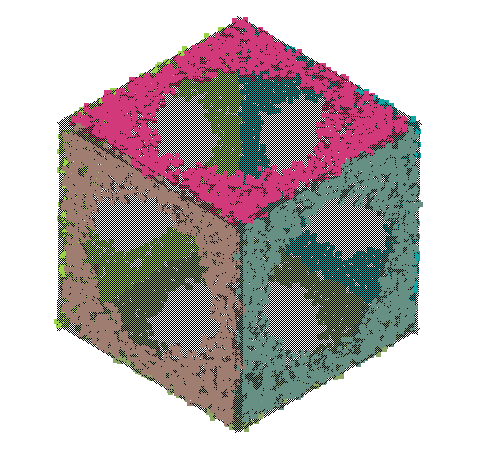
\includegraphics[width=0.9\linewidth]{python/plots/cube_points/data/matrix/cube_points_m6_n01_primitives}
        \caption{Missing level 6}
    \end{subfigure}%
    \begin{subfigure}[b]{0.25\textwidth}
        \centering
        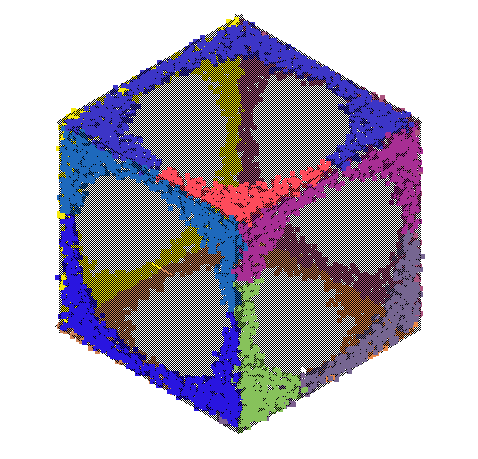
\includegraphics[width=0.9\linewidth]{python/plots/cube_points/data/matrix/cube_points_m12_n01_primitives}
        \caption{Missing level 12}
    \end{subfigure}%
    \begin{subfigure}[b]{0.25\textwidth}
        \centering
        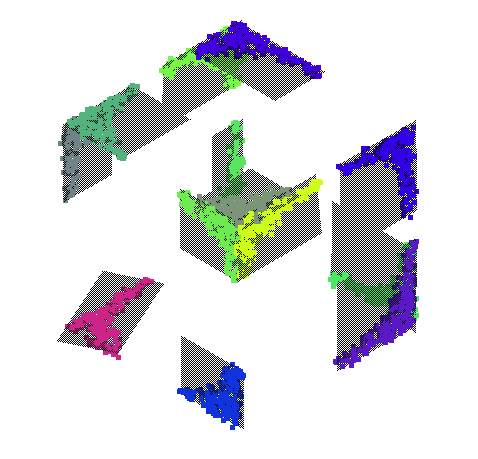
\includegraphics[width=0.9\linewidth]{python/plots/cube_points/data/matrix/cube_points_m24_n01_primitives}
        \caption{Missing level 24}
    \end{subfigure}%
    \caption{Unit cube with noise level = 0.01 and varying missing level}
    \label{fig:test-both}
\end{figure}

\subsection{Tests on real world data}
